\section{Insigts from Information Lattice calculations}

\begin{figure}[h]
    \centering
    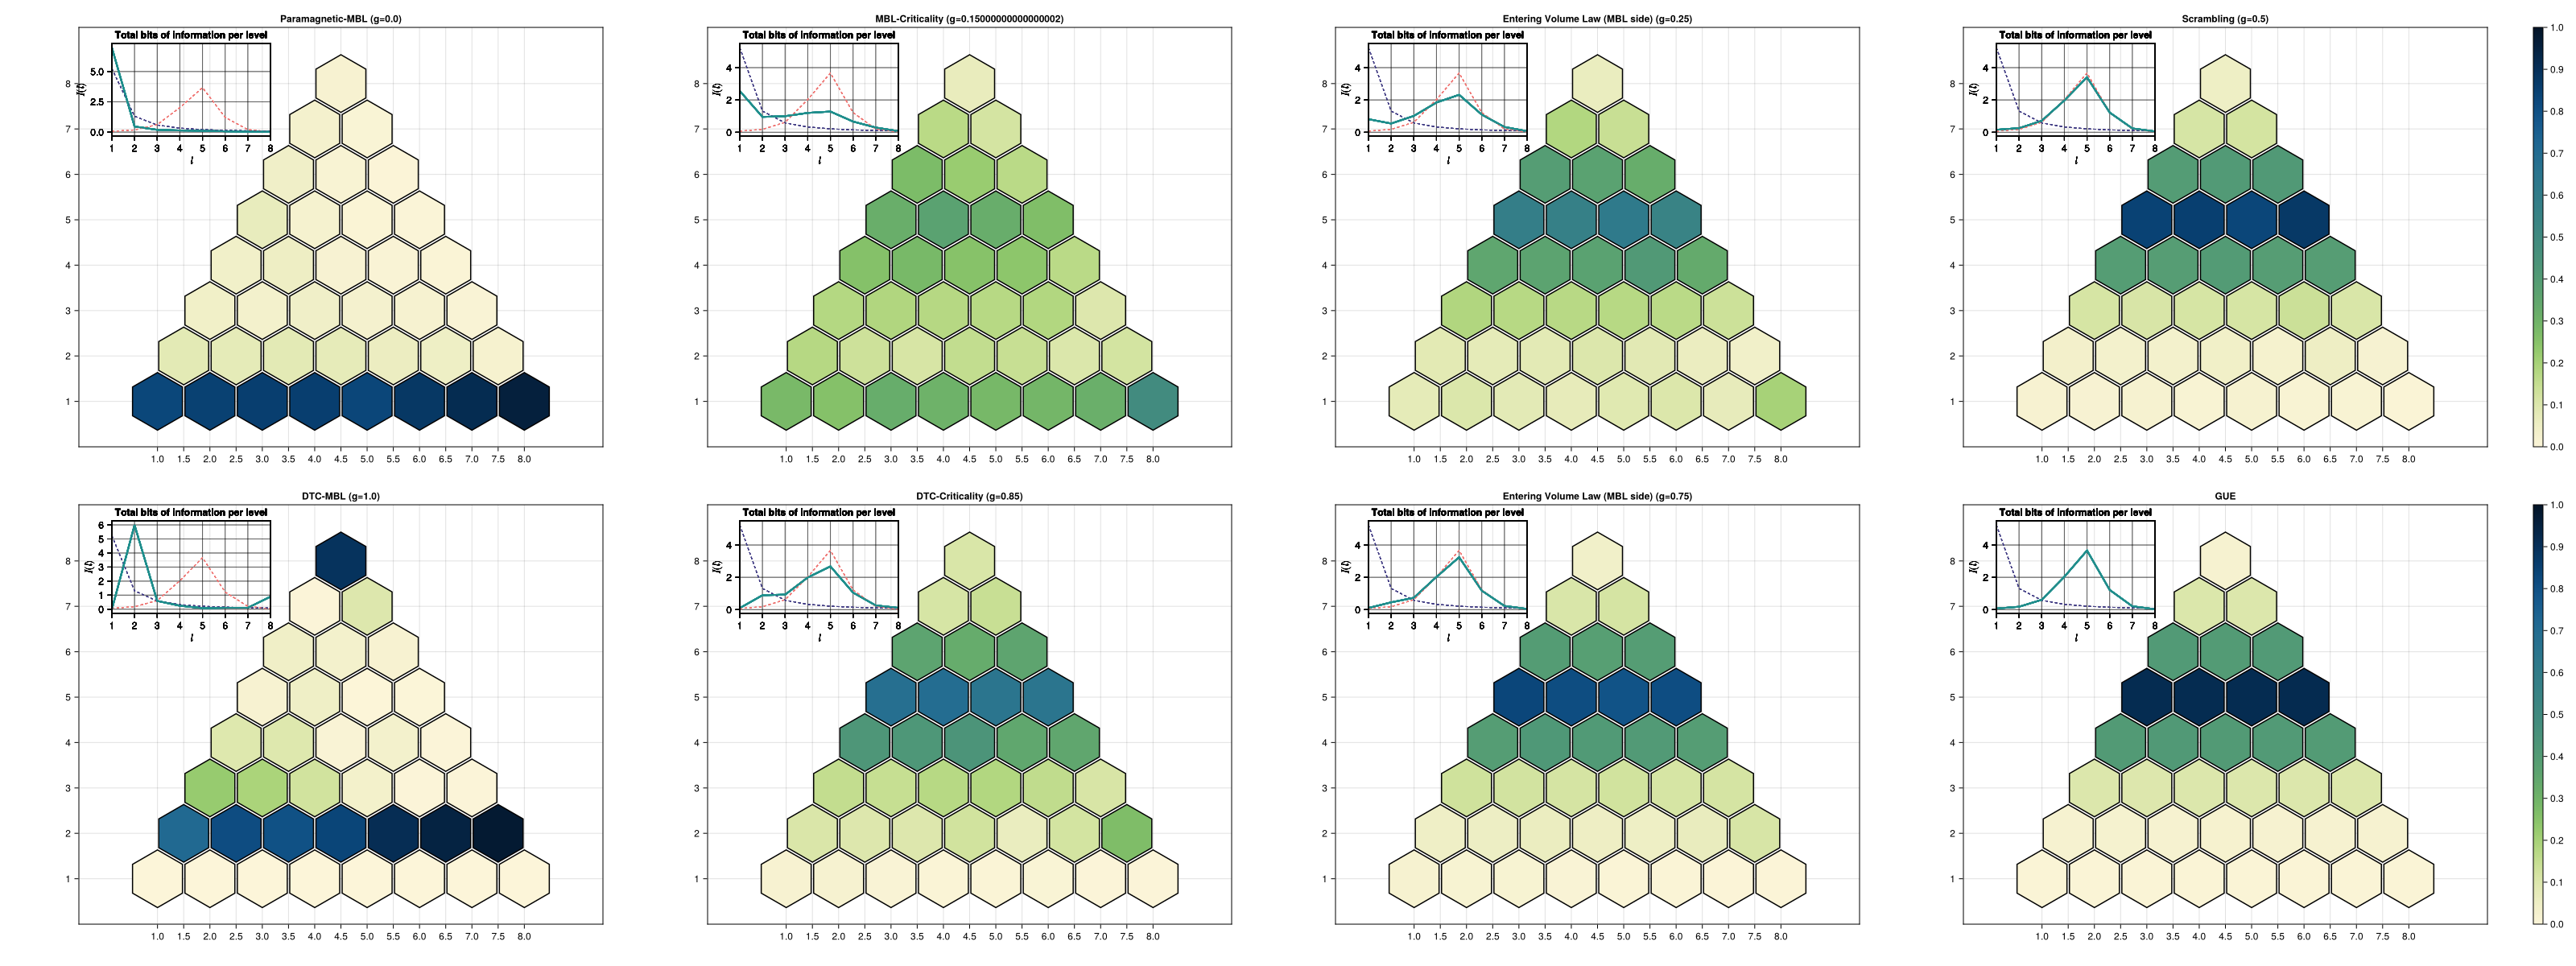
\includegraphics[width=\textwidth]{.src/images/info_lattice_diagram_timecrystals.png}
    \caption{Information Lattice diagram for the time-crystalline circuit: showing the mutual information values for different parameter combinations. The color intensity represents the magnitude of the mutual information, with darker shades indicating higher values. This diagram helps visualize how information is distributed across various length scales of the system.}
    \label{fig:info_lattice_diagram_timecrystals}
\end{figure}



\begin{figure}[h]
    \centering
    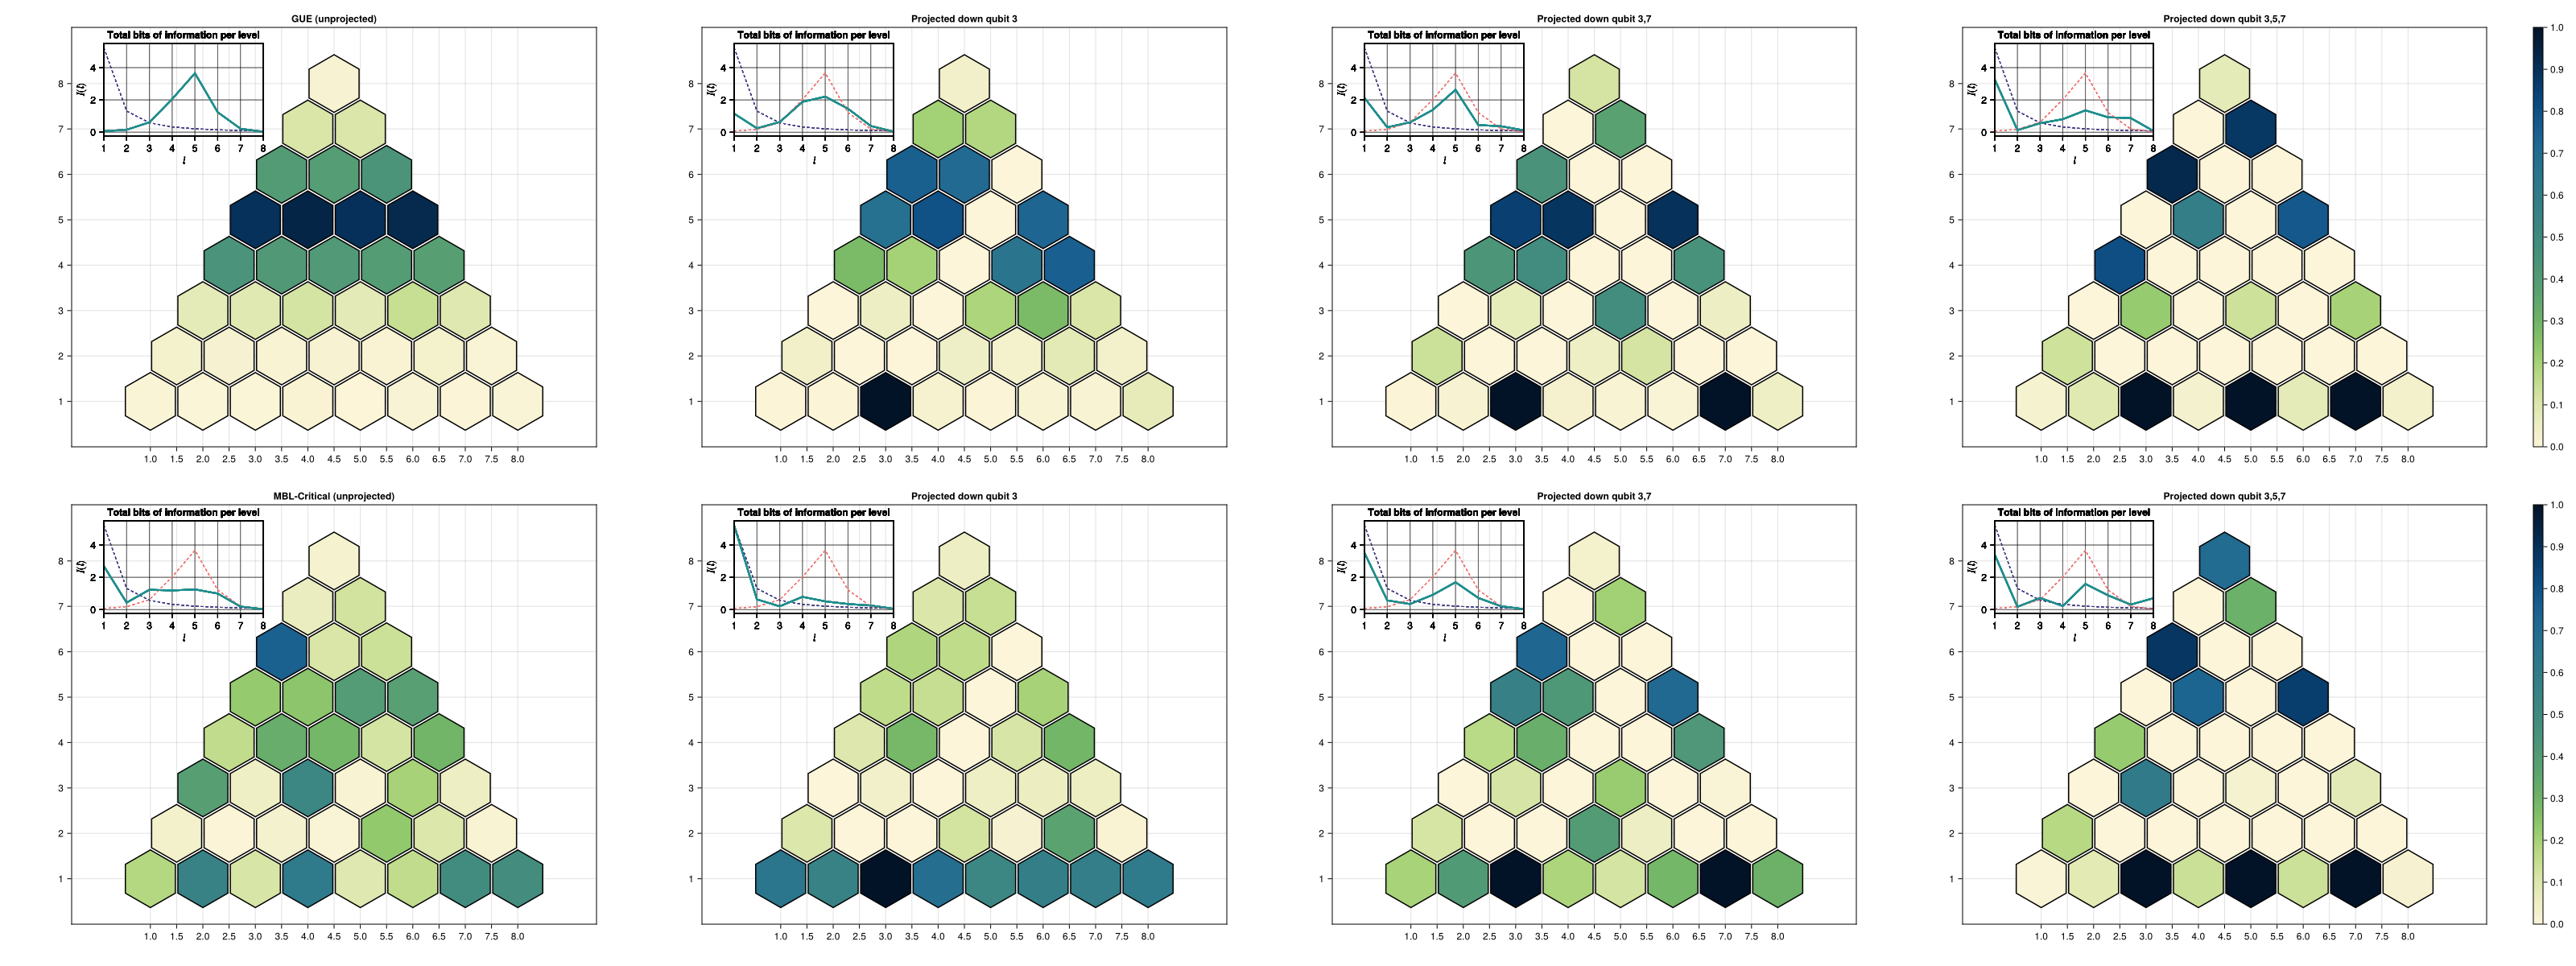
\includegraphics[width=\textwidth]{.src/images/info_lattice_diagram_projections.png}
    \caption{Information Lattice diagram for the ETH-MBL Critical state of the time crystalline circuit (top panel) and GUE (bottom panel) under \textbf{a:}\ no projections ,\textbf{b:}\ projections at site 3, \textbf{c:}\ site 3,5,\textbf{d:}\ site 3,5,7.}
    \label{fig:info_lattice_diagram_projections}
\end{figure}